\documentclass[tikz,border=2mm]{standalone}

\usepackage{tikz}
\usetikzlibrary{positioning,calc}

\begin{document}

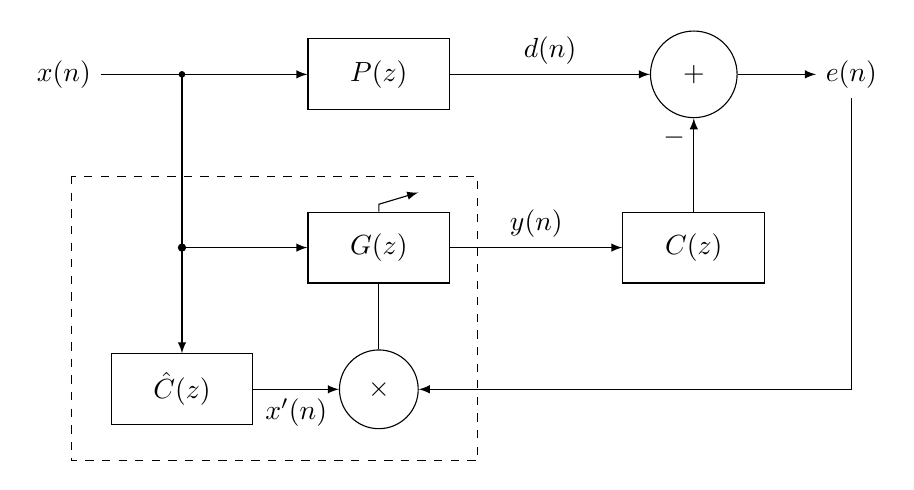
\begin{tikzpicture}[
    block/.style={draw, rectangle, minimum width=18mm, minimum height=9mm},
    sum/.style={draw, circle, minimum size=11mm},
    mult/.style={draw, circle, minimum size=10mm},
    >=latex
]

% Main nodes
\node (x) at (0,0) {$x(n)$};
\node[block] (P) at (4.0,0) {$P(z)$};
\node[sum] (sum) at (8,0) {$+$};
\node (e) at (10,0) {$e(n)$};

\node[block] (G) at (4.0,-2.2) {$G(z)$};
\node[block] (C) at (8,-2.2) {$C(z)$};

\node[block] (Chat) at (1.5,-4.0) {$\hat{C}(z)$};
\node[mult] (mul) at (4,-4.0) {$\times$};

% Helper coordinates
\coordinate (xsplit) at (1.5,0);
\coordinate (xmid) at (1.5,-2.2);
\coordinate (xlow) at (1.5,-2.2);
\coordinate (efb1) at (8.9,-4.0);
\coordinate (upd) at (4.0,-1.65);
\coordinate (updend) at (4.5,-1.5);

% Reference input and split
\draw[-] (x) -- (xsplit);
\fill (xsplit) circle (1.2pt);

\draw[->] (xsplit) -- (P.west);
\draw[-]  (xsplit) -- (xmid);
\draw[->] (xmid) -- (G.west);
\draw[->] (xlow) -- (Chat.north);

\fill (xlow) circle (1.5pt);

% Primary path
\draw[->] (P) -- node[above] {$d(n)$} (sum);

% Secondary path
\draw[->] (G) -- node[above] {$y(n)$} (C);
\draw[->] (C.north) -- (sum.south);

% Error output and feedback
\draw[->] (sum) -- (e);
\draw[-] (e) |- (efb1);
\draw[->] (efb1) -- (mul.east);

% Filtered-x branch
\draw[->] (Chat.east) -- node[below] {$x'(n)$} (mul.west);

% Adaptation update
\draw[-] (mul.north) --  (G.south);
\draw[->] (G.north) -- (upd) -- (updend);

% Minus sign outside summing circle
\node at ($(sum.south)+(-0.25,-0.25)$) {$-$};

% Dashed adaptive block
\draw[dashed]
    ($(Chat.north west)+(-0.5,2.25)$)
    rectangle
    ($(mul.south east)+(0.9,-0.55)$);

\end{tikzpicture}

\end{document}